\documentclass[../../main.tex]{subfiles}

\graphicspath{{../../image/}{../../figure/}}

\begin{document}

\section{坐标变换与迹定理}\label{section:ch01-坐标变换与迹定理}

只要场按适当的规则变换，平衡律场方程的散度形式在坐标变换下保持；事实上，即使通量场仅局部可积，这一结论仍成立。

\begin{theorem}\label{theorem:ch01-坐标变换}
设 $\mathscr{X}$ 为 $\mathbb{R}^{k}$ 的开子集，设 $A\in L^{1}_{\mathrm{loc}}(\mathscr{X};\mathbb{M}^{1\times k})$ 与 $\mathscr{P}\in\mathscr{M}(\mathscr{X})$ 满足场方程
\begin{align}
\operatorname{div} A=\mathscr{P},\label{align:ch01-field-eq}
\end{align}
在 $\mathscr{X}$ 上分布意义下。考虑任一 $\mathscr{X}$ 到 $\mathbb{R}^{k}$ 中子集 $\mathscr{X}^{*}$ 的双 Lipschitz 同胚 $X^{*}$，其 Jacobi 矩阵为
\begin{align}
J=\frac{\partial X^{*}}{\partial X}\label{align:ch01-jacobian}
\end{align}
满足
\begin{align}
\det J\geqslant a>0,\qquad\text{a.e. 在 }\mathscr{X}\text{ 上}.\label{align:ch01-detJ}
\end{align}
则由下式定义的 $A^{*}\in L^{1}_{\mathrm{loc}}(\mathscr{X}^{*};\mathbb{M}^{1\times k})$ 与 $\mathscr{P}^{*}\in\mathscr{M}(\mathscr{X}^{*})$：
\begin{align}
A^{*}\circ X^{*}=(\det J)^{-1}AJ^{\top},\label{align:ch01-A-star}
\end{align}
\begin{align}
\langle\mathscr{P}^{*},\varphi^{*}\rangle=\langle\mathscr{P},\varphi\rangle,\qquad\text{其中 }\varphi=\varphi^{*}\circ X^{*},\label{align:ch01-P-star}
\end{align}
满足场方程
\begin{align}
\operatorname{div} A^{*}=\mathscr{P}^{*},\label{align:ch01-divA-star}
\end{align}
在 $\mathscr{X}^{*}$ 上分布意义下。
\end{theorem}

\begin{proof}
由\cref{align:ch01-field-eq} 得
\begin{align}
\int_{\mathscr{X}}A\,\operatorname{grad}\varphi\,\mathrm{d}X+\langle\mathscr{P},\varphi\rangle=0,\label{align:ch01-dual}
\end{align}
对任一在 $\mathscr{X}$ 中具紧支集的 Lipschitz 函数 $\varphi$ 成立，因为总可构造检验函数序列 $\{\varphi_{m}\}\subset C_{0}^{\infty}(\mathscr{X})$，支集在 $\mathscr{X}$ 的一个紧子集内，使得当 $m\to\infty$ 时，$\varphi_{m}\to\varphi$ 一致收敛，且 $\operatorname{grad}\varphi_{m}\to\operatorname{grad}\varphi$ 在 $\mathscr{X}$ 上几乎处处有界收敛。

给定任一检验函数 $\varphi^{*}\in C_{0}^{\infty}(\mathscr{X}^{*})$，考虑函数 $\varphi=\varphi^{*}\circ X^{*}$，它在 $\mathscr{X}$ 中 Lipschitz 且具紧支集。注意 $\operatorname{grad}\varphi=J^{\top}\operatorname{grad}\varphi^{*}$。此外 $\mathrm{d}X^{*}=(\det J)\,\mathrm{d}X$。借助这些关系以及\cref{align:ch01-A-star,align:ch01-P-star}，可将\cref{align:ch01-dual} 写为
\begin{align}
\int_{\mathscr{X}^{*}}A^{*}\,\operatorname{grad}\varphi^{*}\,\mathrm{d}X^{*}+\langle\mathscr{P}^{*},\varphi^{*}\rangle=0,\label{align:ch01-dual-star}
\end{align}
这就证明了\cref{align:ch01-divA-star}。证明完成。
\end{proof}

\begin{remark}\label{remark:ch01-密度变换}
在\cref{align:ch01-production-density} 所刻画的常见特殊情形中，测度 $\mathscr{P}$ 由生成密度场 $p\in L^{1}_{\mathrm{loc}}(\mathscr{X})$ 诱导，\cref{align:ch01-P-star} 蕴涵 $\mathscr{P}^{*}$ 也由生成密度场 $p^{*}\in L^{1}_{\mathrm{loc}}(\mathscr{X}^{*})$ 诱导，其表达式为
\begin{align}
p^{*}\circ X^{*}=(\det J)^{-1}p.\label{align:ch01-p-star}
\end{align}
\end{remark}

尽管一般地场 $A$ 仅在 $\mathbb{R}^{k}$ 的开子集上几乎处处有定义，但场方程却诱导出一定程度的正则性，体现在迹定理中；这使我们能够识别通过余维 $1$ 曲面的通量，从而恢复原始形式的平衡律。先从平面曲面开始。

\begin{lemma}\label{lemma:ch01-平面迹}
假设 $A\in L^{\infty}(\mathscr{K};\mathbb{M}^{1\times k})$ 与 $\mathscr{P}\in\mathscr{M}(\mathscr{K})$ 在柱域 $\mathscr{K}=\mathscr{B}\times(\alpha,\beta)$ 上满足\cref{align:ch01-field-eq}（分布意义），其中 $\mathscr{B}$ 为 $\mathbb{R}^{k-1}$ 中的球。设 $E_{k}$ 为 $\mathbb{R}^{k}$ 中的第 $k$ 个基向量，记 $X=(x,t)$，其中 $x\in\mathscr{B}$、$t\in(\alpha,\beta)$。则在必要于一零测集上修改 $A$ 之后，函数 $a(x,t)=A(x,t)E_{k}$ 具有以下性质：单侧极限 $a(\cdot,\tau\pm)$ 在 $L^{\infty}(\mathscr{B})$ 弱$^{*}$ 意义下对任意 $\tau\in(\alpha,\beta)$ 存在，并可由下式确定
\begin{align}
\begin{cases}
a(x,\tau-)=\displaystyle\operatorname*{ess\,lim}_{t\uparrow\tau}A(x,t)E_{k}=\lim_{\varepsilon\downarrow 0}\frac{1}{\varepsilon}\int_{\tau-\varepsilon}^{\tau}A(x,t)E_{k}\,\mathrm{d}t,\\[2mm]
a(x,\tau+)=\displaystyle\operatorname*{ess\,lim}_{t\downarrow\tau}A(x,t)E_{k}=\lim_{\varepsilon\downarrow 0}\frac{1}{\varepsilon}\int_{\tau}^{\tau+\varepsilon}A(x,t)E_{k}\,\mathrm{d}t,
\end{cases}\label{align:ch01-trace-one-sided}
\end{align}
其中极限在 $L^{\infty}(\mathscr{B})$ 弱$^{*}$ 意义下取。此外，对任意 $\tau\in(\alpha,\beta)$ 与任一在 $\mathscr{K}$ 中具紧支集的 Lipschitz 连续函数 $\varphi$，
\begin{align}
\begin{cases}
\displaystyle\int_{\mathscr{B}}a(x,\tau-)\varphi(x,\tau)\,\mathrm{d}x
=\int_{\mathscr{B}\times(\alpha,\tau)}A(X)\operatorname{grad}\varphi(X)\,\mathrm{d}X+\langle\mathscr{P},\varphi\rangle_{\mathscr{B}\times(\alpha,\tau)},\\[2mm]
\displaystyle-\int_{\mathscr{B}}a(x,\tau+)\varphi(x,\tau)\,\mathrm{d}x
=\int_{\mathscr{B}\times(\tau,\beta)}A(X)\operatorname{grad}\varphi(X)\,\mathrm{d}X+\langle\mathscr{P},\varphi\rangle_{\mathscr{B}\times(\tau,\beta)}.
\end{cases}\label{align:ch01-trace-identity}
\end{align}
于是 $a(\cdot,\tau-)=a(\cdot,\tau+)=a(\cdot,\tau)$，除非 $\tau$ 属于使 $|\mathscr{P}|(\mathscr{B}\times\{\tau\})>0$ 的（至多可数）点集。特别地，当 $\mathscr{P}$ 关于 Lebesgue 测度绝对连续时，函数 $\tau\mapsto a(\cdot,\tau)$ 在 $(\alpha,\beta)$ 上按 $L^{\infty}(\mathscr{B})$ 的弱$^{*}$ 拓扑连续。
\end{lemma}

\begin{proof}
取正的小量 $\varepsilon$。设 $r$ 为 $\mathscr{B}$ 的半径，记 $\mathscr{B}_{\varepsilon}$ 为 $\mathbb{R}^{k-1}$ 中与 $\mathscr{B}$ 同心、半径为 $r-\varepsilon$ 的球。如\cref{theorem:ch01-场方程归约} 的证明中那样，通过\cref{align:ch01-mollified} 在 $\mathscr{B}_{\varepsilon}\times(\alpha+\varepsilon,\beta-\varepsilon)$ 上磨光 $A$ 与 $\mathscr{P}$。所得光滑场 $A_{\varepsilon}$ 与 $p_{\varepsilon}$ 满足\cref{align:ch01-divAeps-equality}。再令 $a_{\varepsilon}(x,t)=A_{\varepsilon}(x,t)E_{k}$。

以 $\mathscr{B}_{\varepsilon}$ 上具紧支集的 Lipschitz 函数 $\varphi$ 乘\cref{align:ch01-divAeps-equality}，并在 $\mathscr{B}_{\varepsilon}\times(r,s)$ 上积分，其中 $\alpha+\varepsilon<r<s<\beta-\varepsilon$。分部积分后得到
\begin{align}
\begin{aligned}
\int_{\mathscr{B}_{\varepsilon}}a_{\varepsilon}(x,s)\varphi(x)\,\mathrm{d}x-\int_{\mathscr{B}_{\varepsilon}}a_{\varepsilon}(x,r)\varphi(x)\,\mathrm{d}x
=\int_{r}^{s}\int_{\mathscr{B}_{\varepsilon}}\bigl\{A_{\varepsilon}(x,t)\Pi_{k}\operatorname{grad}\varphi(x)+p_{\varepsilon}(x,t)\varphi(x)\bigr\}\,\mathrm{d}x\,\mathrm{d}t,
\end{aligned}\label{align:ch01-mollified-integrated}
\end{align}
其中 $\Pi_{k}$ 表示 $\mathbb{R}^{k}$ 到 $\mathbb{R}^{k-1}$ 的投影。由此，函数 $t\mapsto\int_{\mathscr{B}_{\varepsilon}}a_{\varepsilon}(x,t)\varphi(x)\,\mathrm{d}x$ 在区间 $(\alpha+\varepsilon,\beta-\varepsilon)$ 上的全变差关于 $\varepsilon>0$ 一致有界。因此，从 $\mathscr{B}_{\varepsilon}$ 中具紧支集、在 $L^{1}(\mathscr{B})$ 中稠密的可数检验函数族 $\{\varphi_{\ell}\}$ 出发，可借助 Helly 定理与对角论证提取一列 $\{\varepsilon_{m}\}$，$\varepsilon_{m}\to 0$（$m\to\infty$），并确定 $(\alpha,\beta)$ 的一个可数子集 $G$，使得对任意 $\ell=1,2,\cdots$，序列 $\{\int_{\mathscr{B}}a_{\varepsilon_{m}}(x,t)\varphi_{\ell}(x)\,\mathrm{d}x\}$ 当 $m\to\infty$ 时对每个 $t\in(\alpha,\beta)\setminus G$ 收敛，且极限函数在 $(\alpha,\beta)$ 上有界变差。对所有 $\ell$ 所得极限函数可统一表为 $\int_{\mathscr{B}}a(x,t)\varphi_{\ell}(x)\,\mathrm{d}x$，其中某函数 $t\mapsto a(\cdot,t)$ 取值于 $L^{\infty}(\mathscr{B})$。显然在 $\mathscr{K}$ 上 a.e. 有 $a(x,t)=A(x,t)E_{k}$。故 $a$ 不依赖于构造时所用的特定序列 $\{\varepsilon_{m}\}$，且\cref{align:ch01-trace-one-sided} 对任意 $\tau\in(\alpha,\beta)$ 成立。

给定任一 $\tau\in(\alpha,\beta)$ 与任一在 $\mathscr{K}$ 中具紧支集的 Lipschitz 函数 $\varphi$，以 $\varphi$ 乘\cref{align:ch01-divAeps-equality} 并在 $\mathscr{B}_{\varepsilon}\times(\alpha+\varepsilon,s)$ 上积分，其中 $s\in(\alpha+\varepsilon,\tau)\setminus G$。分部积分后得到
\begin{align}
\int_{\mathscr{B}_{\varepsilon}}a_{\varepsilon}(x,s)\varphi(x,s)\,\mathrm{d}x=\int_{\mathscr{B}_{\varepsilon}\times(a+\varepsilon,s)}\bigl[A_{\varepsilon}(X)\operatorname{grad}\varphi(X)+p_{\varepsilon}(X)\varphi(X)\bigr]\,\mathrm{d}X.\label{align:ch01-pass-to-limit}
\end{align}
在\cref{align:ch01-pass-to-limit} 中先令 $\varepsilon\downarrow 0$ 再令 $s\uparrow\tau$，即得到\cref{align:ch01-trace-identity} 的第一式；第二式证明类似。

当 $\mathscr{P}$ 关于 Lebesgue 测度绝对连续时，\cref{align:ch01-mollified-integrated} 蕴涵以 $\varepsilon$ 为参数的函数族 $t\mapsto\int_{\mathscr{B}_{\varepsilon}}a_{\varepsilon}(x,t)\varphi_{\ell}(x)\,\mathrm{d}x$ 实际上等度连续，从而 $\int_{\mathscr{B}}a(x,t)\varphi_{\ell}(x)\,\mathrm{d}x$ 在 $(\alpha,\beta)$ 上连续，对任意 $\ell=1,2,\cdots$。于是 $t\mapsto a(\cdot;t)$ 在 $(\alpha,\beta)$ 上 $L^{\infty}(\mathscr{B})$ 弱$^{*}$ 连续。证明完成。
\end{proof}

上述命题中特意突出第 $k$ 坐标方向只是为方便。显然 $AE_{\alpha}$ 沿任一基向量 $E_{\alpha}$ 的方向、乃至 $AN$ 沿任一 $N\in\mathbb{S}^{k-1}$ 的方向，都具有类似的连续性。因此，从场方程\cref{align:ch01-divA-P} 出发，可以恢复\cref{theorem:ch01-场方程归约} 中出现的平面曲面的密度通量函数 $a_{N}$。下述命题表明，一般真域 $\mathscr{D}$ 的密度通量函数 $q_{\mathscr{D}}$ 也可由同一程序恢复。

\begin{theorem}\label{theorem:ch01-一般迹}
假设 $A\in L^{\infty}(\mathscr{X};\mathbb{M}^{1\times k})$ 与 $\mathscr{P}\in\mathscr{M}(\mathscr{X})$ 在 $\mathbb{R}^{k}$ 的开子集 $\mathscr{X}$ 上满足\cref{align:ch01-field-eq}（分布意义）。则对 $\mathscr{X}$ 中任一真域 $\mathscr{D}$，伴随一个 $\partial\mathscr{D}$ 上有界、$\mathscr{H}^{k-1}$-可测的函数 $q_{\mathscr{D}}$，使得对任一在 $\mathbb{R}^{k}$ 上 Lipschitz 连续、在 $\mathscr{X}$ 中具紧支集的函数 $\varphi$，
\begin{align}
\int_{\partial\mathscr{D}}q_{\mathscr{D}}(X)\varphi(X)\,\mathrm{d}\mathscr{H}^{k-1}(X)=\int_{\mathscr{D}}A(X)\operatorname{grad}\varphi(X)\,\mathrm{d}X+\langle\mathscr{P},\varphi\rangle_{\mathscr{D}}.\label{align:ch01-general-trace}
\end{align}

\end{theorem}

\begin{figure}[ht]
\centering
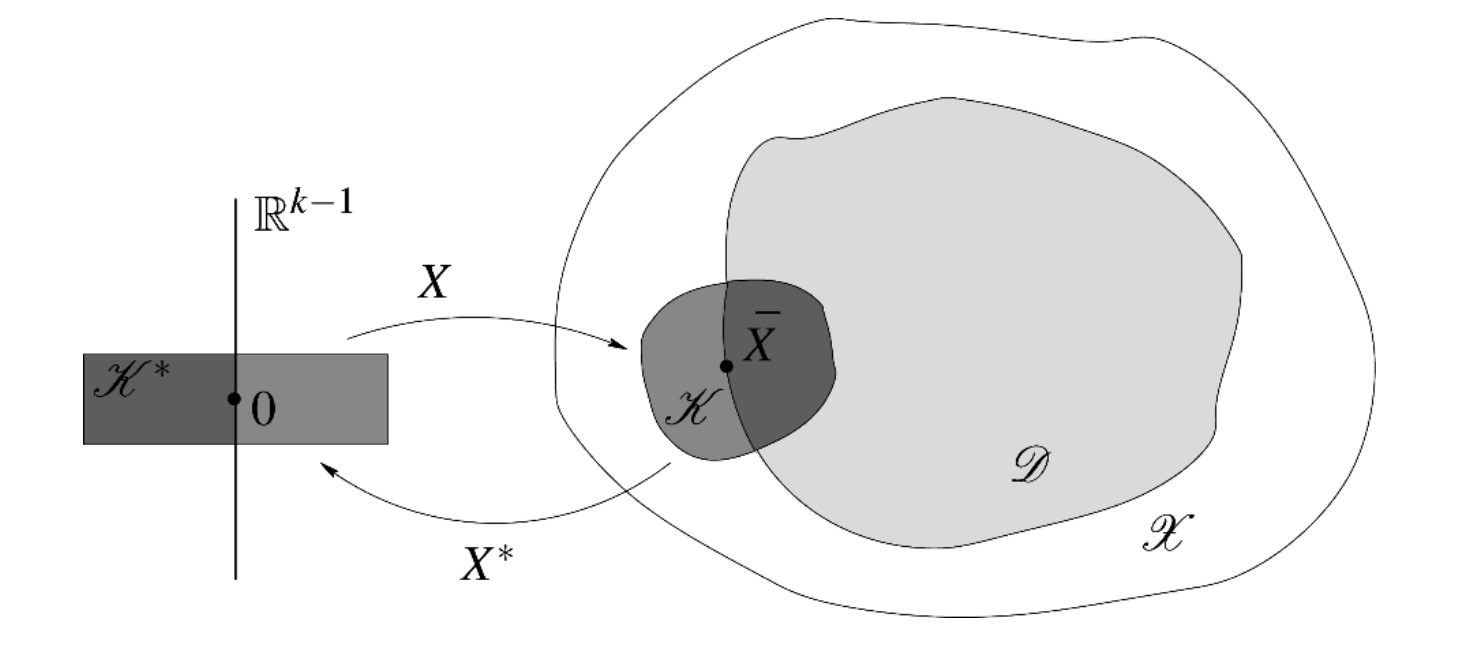
\includegraphics[width=0.85\textwidth]{../../image/ch01-fig03-01.png}
\caption{通过双 Lipschitz 同胚 $X:\mathscr{K}^{*}\to\mathscr{K}$ 局部化迹。}\label{figure:ch01-localization}
\end{figure}

\begin{proof}
考虑柱域 $\mathscr{K}^{*}=\{X^{*}=(x,t):x\in\mathscr{B},\ t\in(-1,1)\}$，其中 $\mathscr{B}$ 为 $\mathbb{R}^{k-1}$ 中的单位球。固定 $\mathscr{X}$ 中任一真域 $\mathscr{D}$。

由于 $\mathscr{D}$ 是 Lipschitz 域，对每一点 $\bar{X}\in\partial\mathscr{D}$，伴随一个从 $\mathscr{K}^{*}$ 到 $\mathscr{X}$ 中某开子集 $\mathscr{K}$ 的双 Lipschitz 同胚 $X$，使得 $X(0)=\bar{X}$、$X(\mathscr{B}\times(-1,0))=\mathscr{D}\cap\mathscr{K}$ 且 $X(\mathscr{B}\times\{0\})=\partial\mathscr{D}\cap\mathscr{K}$；见\cref{figure:ch01-localization}。

考虑 $X$ 的逆映射 $X^{*}$，其 Jacobi 矩阵 $J$ 由\cref{align:ch01-jacobian} 给出并满足\cref{align:ch01-detJ}。通过\cref{align:ch01-A-star} 构造 $A^{*}\in L^{\infty}(\mathscr{K}^{*};\mathbb{M}^{1\times k})$，通过\cref{align:ch01-P-star} 构造 $\mathscr{P}^{*}\in\mathscr{M}(\mathscr{K}^{*})$，二者在 $\mathscr{K}^{*}$ 上分布意义下满足\cref{align:ch01-divA-star}。

现应用\cref{lemma:ch01-平面迹} 来确定 $\mathscr{K}^{*}$ 上的函数 $a^{*}(x,t)$，它在 $\mathscr{K}^{*}$ 上 a.e. 等于 $A^{*}(x,t)E_{k}$，并由\cref{align:ch01-trace-one-sided} 满足
\begin{align}
a^{*}(x,0-)=\operatorname*{ess\,lim}_{t\to 0}A^{*}(x,t)E_{k}=\lim_{\varepsilon\downarrow 0}\frac{1}{\varepsilon}\int_{-\varepsilon}^{0}A^{*}(x,t)E_{k}\,\mathrm{d}t.\label{align:ch01-a-star-trace}
\end{align}

固定任一在 $\mathbb{R}^{k}$ 上 Lipschitz 连续、在 $\mathscr{K}$ 中具紧支集的函数 $\varphi$，令 $\varphi^{*}=\varphi\circ X$，$X^{*}\in\mathscr{K}^{*}$。借助\cref{align:ch01-trace-identity}，
\begin{align}
\int_{\mathscr{B}}a^{*}(x,0-)\varphi^{*}(x,0)\,\mathrm{d}x=\int_{\mathscr{B}\times(-1,0)}A^{*}(X^{*})\operatorname{grad}\varphi^{*}(X^{*})\,\mathrm{d}X^{*}+\langle\mathscr{P}^{*},\varphi^{*}\rangle_{\mathscr{B}\times(-1,0)}.\label{align:ch01-a-star-identity}
\end{align}

利用同胚 $X^{*}$ 将\cref{align:ch01-a-star-identity} 变换为 $\mathscr{X}$ 上的方程。由 $\operatorname{grad}\varphi=J^{\top}\operatorname{grad}\varphi^{*}$，并回忆\cref{align:ch01-A-star,align:ch01-P-star}，可将\cref{align:ch01-a-star-identity} 重写为
\begin{align}
\int_{\partial\mathscr{D}\cap\mathscr{K}}q_{\mathscr{D}}(X)\varphi(X)\,\mathrm{d}\mathscr{H}^{k-1}(X)=\int_{\mathscr{D}}A(X)\operatorname{grad}\varphi(X)\,\mathrm{d}X+\langle\mathscr{P},\varphi\rangle_{\mathscr{D}},\label{align:ch01-local-trace}
\end{align}
其中已令
\begin{align}
q_{\mathscr{D}}=\frac{\mathrm{d}x}{\mathrm{d}\mathscr{H}^{k-1}}a^{*}\circ X^{*}=\frac{\det J}{E_{k}^{\top}JN}a^{*}\circ X^{*},\label{align:ch01-qD-formula}
\end{align}
$N$ 表示 $\mathscr{D}$ 的外单位法向。

\cref{align:ch01-local-trace} 确立了\cref{align:ch01-general-trace}，但此时仅对支集在 $\mathscr{K}$ 中的 $\varphi$ 成立。然而应注意，\cref{align:ch01-local-trace} 的右端不依赖于同胚 $X^{*}$，因此 $q_{\mathscr{D}}$ 在 $\partial\mathscr{D}\cap\mathscr{K}$ 上的值是内在定义的，独立于上述具体构造。于是，通过直截了当的单位分解论证，容易从\cref{align:ch01-local-trace} 过渡到对任意在 $\mathscr{X}$ 中具紧支集的 Lipschitz 连续函数 $\varphi$ 成立的\cref{align:ch01-general-trace}。证明完成。
\end{proof}

在\cref{section:ch01-注记} 所引文献中，读者可找到上述命题的更精细版本：其中 $A$ 仅假定局部可积甚至只是一个测度，并给出替代的证明方法。例如，在更抽象的途径中，通过证明\cref{align:ch01-general-trace} 的右端可实现为 $L^{1}(\partial\mathscr{D})$ 上的有界线性泛函来确立 $q_{\mathscr{D}}$ 的存在性。

\begin{remark}\label{remark:ch01-显式迹构造}
在理论的应用中，常需要从 $A$ 显式构造 $q_{\mathscr{D}}$。对几何结构简单的域 $\mathscr{D}$，这很容易得到。首先，当 $\mathscr{D}$ 是某 $N\in\mathbb{S}^{k-1}$ 对应的半空间 $\{X\in\mathbb{R}^{k}:X\cdot N<0\}$ 时，\cref{lemma:ch01-平面迹} 蕴涵
\begin{align}
q_{\mathscr{D}}(X)=\operatorname*{ess\,lim}_{t\to 0}A(X-tN)N=\lim_{\varepsilon\to 0}\frac{1}{\varepsilon}\int_{0}^{\varepsilon}A(x-tN)N\,\mathrm{d}t,\label{align:ch01-halfspace-trace}
\end{align}
极限在 $L^{\infty}(\mathbb{R}^{k-1})$ 弱$^{*}$ 意义下取。其次考虑具有如下性质的任一 $\mathscr{D}$：对每个 $X_{0}\in\partial\mathscr{D}$，伴随 $r>0$、$\varepsilon_{0}>0$ 与 $N\in\mathbb{S}^{k-1}$，使得对集合 $\mathscr{C}=\partial\mathscr{D}\cap\mathscr{B}_{r}(X_{0})$ 中所有 $X$ 与 $t\in(0,\varepsilon_{0})$，点 $X-tN$ 落在 $\mathscr{D}$ 内。于是，将\cref{align:ch01-general-trace} 应用于沿 $-N$ 方向由 $\mathscr{C}$ 的平移叶状化的检验函数 $\varphi$，我们推出\cref{align:ch01-halfspace-trace} 对 $\mathscr{C}$ 中 $X$ 成立，此时极限在 $L^{\infty}(\mathscr{C})$ 弱$^{*}$ 意义下取。
\end{remark}

\end{document}
